% 
% Annual Cognitive Science Conference
% Sample LaTeX Paper -- Proceedings Format
% \


% to do
% -- consistent names of conditions: listener uncertainty in common ground vs. not
% -----

\documentclass[10pt,letterpaper]{article}

\usepackage{cogsci}
\usepackage{pslatex}
\usepackage{apacite}
\usepackage{url}
\usepackage{graphicx}
\usepackage{caption}
\usepackage{subcaption}
\usepackage{listings}
\usepackage{color}
\usepackage{textcomp}
\usepackage{amsmath}
\usepackage{amssymb}
\usepackage{wrapfig}
\usepackage{lipsum}

\graphicspath{{figures/}}

\def\signed #1{{\leavevmode\unskip\nobreak\hfil\penalty50\hskip2em
  \hbox{}\nobreak\hfil(#1)%
  \parfillskip=0pt \finalhyphendemerits=0 \endgraf}}

\newsavebox\mybox
\newenvironment{aquote}[1]
  {\savebox\mybox{#1}\begin{quote}}
  {\signed{\usebox\mybox}\end{quote}}

 \newcommand{\denote}[1]{\mbox{ $[\![ #1 ]\!]$}}

\definecolor{Red}{RGB}{255,0,0}
\newcommand{\red}[1]{\textcolor{Red}{#1}}  

\definecolor{Blue}{RGB}{0,0,255}
\newcommand{\blue}[1]{\textcolor{Blue}{#1}}  

\title{It goes without saying: The pragmatics of uninformative utterances}

\author{{\large \bf Eleanor Chestnut*}, {\large \bf Michael Henry Tessler*},
{\large \bf Ellen M. Markman}, and {\large \bf Noah D. Goodman}  \\
\{eleanor.chestnut, mtessler, markman, ngoodman\} @stanford.edu \\ 
  Department of Psychology, Stanford University \\
  *Authors contributed equally to this publication}

\begin{document}

\maketitle


\begin{abstract}

Language is interpreted in context with respect to some common ground between speaker and listener.
Common ground can make certain utterances uninformative (e.g. stating something obvious), but is plausibly revised in the face of uninformative utterances.
Here, we formalize common ground inference when a speaker's utterance refers to something that should already be in common ground.
The formal pragmatics model predicts that this kind of utterance will backfire (i.e. imply the opposite) when the listener's uncertainty about the common ground is not itself in common ground, but not when that uncertainty is in common ground (e.g. by the listener stating it explicitly). 
%In Expt.~1, we verify this prediction using a paradigm that makes the 


\textbf{Keywords:} 
pragmatics; language; common ground; Bayesian model

\end{abstract}

\section{Introduction}

In one of the most infamous moments in U.S. presidential history, Richard Nixon declared to the press corps, "I am not a crook"€ (CITE).  On the surface, this claim argues for Nixon's innocence, as it literally states that he is not a crook.  As several researchers have shown, however, this statement contains a number of pragmatic implications that actually counter its literal, semantic meaning (CITE).  Nixon'€™s claim, for instance, presupposes that others believed that he was a crook; otherwise, it would not have been an informative statement to make, since most people presumably are not crooks (Grice, 1975).  Thus, if a listener is not aware of the Watergate scandal, or if they have no reason to question Nixon's moral status, they might actually learn from this claim that Nixon was likely corrupt in some way.

\red{not shortening this yet because i think it's better to just write everything out, and then cut in the end of need be.}

To date, this inferential process, or "€œbackfiring"€ linguistic effect, has received little attention in the literature.  In fact, most theories of language processing assert the opposite: if a person hears that Nixon is not a crook, then they should update their belief about Nixon to include this information... \red{EDIT}.  A few studies, however, provide preliminary evidence that utterances that are redundant with a listener'€™s preexisting beliefs do cause listeners to search for ways to make those utterances informative \cite{Yandell1979, Wegner1981, Gruenfeld1992, Kravtchenko2015}.  This process ultimately undermines the utterances' literal meanings.  
\citeA{Wegner1981}, for example, demonstrated that newspaper headlines such as "€œBob Talbert is not linked to the Mafia" [CHECK] cause adults to have a more negative impression of Bob than they would otherwise, despite not explicitly asserting any incriminating information--indeed, despite denying incriminating information.  Here, since the default assumption is that people are not typically linked to the mafia, this headline is not immediately informative.  As a result, adults construct a context that \emph{would} make the headline informative, namely, one in which Bob is known to be a bad person.  
\citeA{Gruenfeld1992} went even further to show that uninformative newspaper headlines can actually cause people to believe the exact opposite of what those headlines claim.  After reading the headline "€œRobert Kennedy was not planning the assassination of Fidel Castro"€, for example, which denies a proposition that adults \emph{a priori} should not believe, adults in their study more strongly believed that Robert Kennedy \emph{was} planning to assassinate Fidel Castro.


\begin{figure}
\centering
    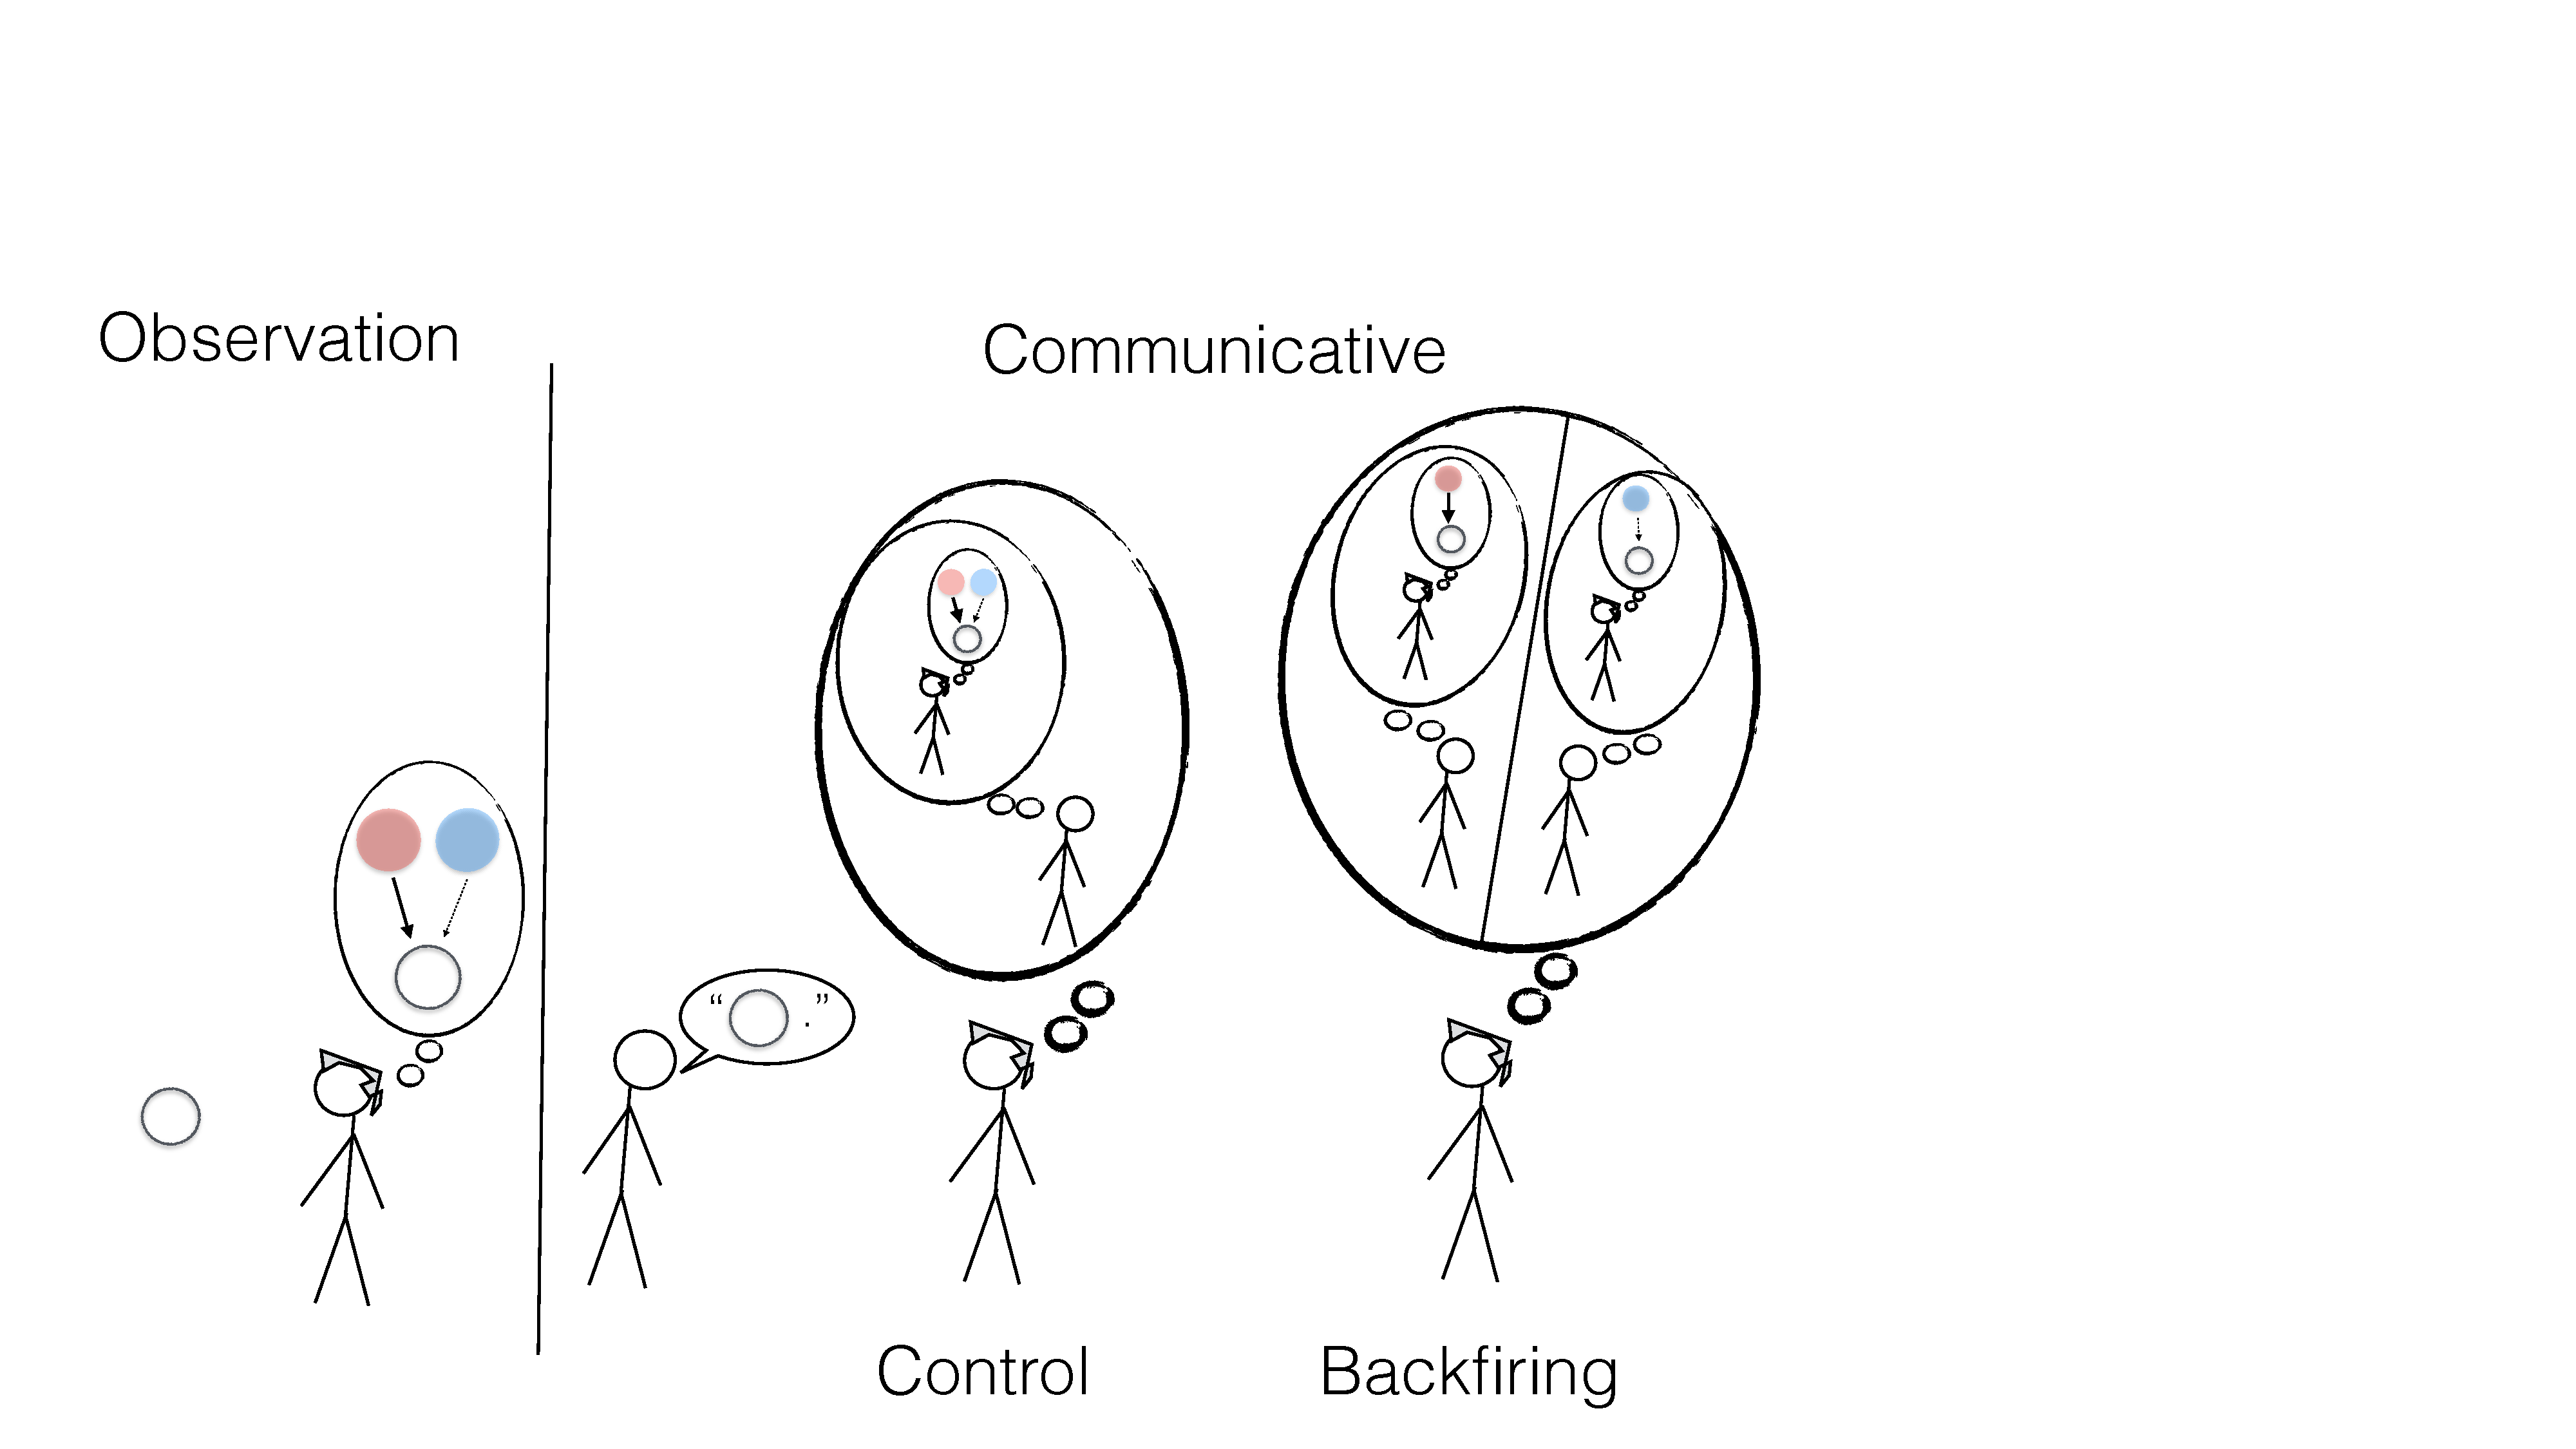
\includegraphics[width=\columnwidth]{cartoon}
    \caption{}
  \label{fig:cartoon}
\end{figure}

\red{I WOULD MOVE THE FIGURE TO THE MODEL SECTION}

Affirming redundant information can have a similar effect \cite{Gruenfeld1992, Kravtchenko2015}.  
\citeA{Kravtchenko2015} for example, recently showed that if a speaker says, "John paid the cashier!" as part of a story about a trip to a grocery store, adults will infer that John does not typically pay cashiers.  This inference is based on the fact that paying cashiers is a standard part of buying groceries, and can easily be inferred without the speaker having to state it explicitly (Bower et al., etc.).  Thus, in an attempt to make the utterance informative, adults assume that paying cashiers must be uncharacteristic of John.  Critically, if the story begins by asserting that John is usually broke, then adults do not make this inference, because the idea of John paying the cashier is no longer redundant with their expectations.

To our knowledge, no current model of language processing can account for this pragmatic inference.  We propose such a model in the present study.  In Experiment 1, we replicate previous findings that adults try to avoid redundancy in conversation by revising their beliefs about the world so that potentially uninformative utterances become informative \cite{Kravtchenko2015} (also cite Jaeger studies etc.).  Specifically, we ask whether utterances such as, "My student turned in her homework on time today,"€ imply that the student does not typically turn in her homework on time, despite serving as evidence for this behavior.  We then test whether our proposed model predicts these results.  We also test an important, previously unexplored(?) prediction of our model: that this "€œbackfiring"€ effect of language should be eliminated 1) when the listener makes explicit her uncertainty, for instance, about whether the student turned in his homework on time, since this would make the speaker's utterance semantically informative; and 2) when the utterance is removed from any conversational context, since this pragmatic inference depends on the \emph{conversational} agreement that utterances should be informative.

\section{A model of backfiring language}

Observing an event is often evidence for an underlying cause that could reliably give rise to the event.
For example, if you are waiting for a bus that ends up being 15 minutes late, it is reasonable to fear it may be late the next day; public transit in this town may be unreliable. 
%disembark in a novel location to find it raining, it is reasonable to fear it may be raining in five minutes. 
%Raining events are correlated with future raining events, and this place might well be a rainy place. 
Similarly, observing a behavior $b$ in a person can be taken as evidence for an underlying habit $h$. 
Seeing your friend's roommate doing her dishes provides some evidence that the roommate usually does her dishes. 
It is a more likely explanation than the alternative.

We can formalize this using a simple Bayesian model:
\begin{align*}
P(h \mid b) & \propto P(b \mid h) P(h) 
\end{align*}
As a habit is more likely to give rise to the behavior --- as $P(b \mid h)$ gets large --- so too does the behavior become more indicative of the habit, assuming the prior probabilities are constant. 

Knowledge of such a causal system may or may not be in common ground, and the corresponding meta-knowledge may or may not as well \cite{Clark1977, Clark1996}. 
For example, in pedagogical situations, it is valid to assume the knowledge of the causal system to be taught is \emph{not} in common ground, but that both teacher and learner have in common ground this fact.
Other communicative settings may exist, where the both levels of knowledge are not in common ground.  \red{I WOULD ADD AN EXAMPLE TO MAKE THIS CLEARER}
When the listener thinks that the speaker is presupposing some knowledge of the causal system, she can use the speech-act to help resolve what the speaker is presupposing to be be in common ground.

This can be readily incorporated into Rational Speech-Acts framework \cite{Frank2012, Goodman2013}:, as a lifted variable inference akin to the treatment by \citeA{Degen2015} and discussed in \citeA{GoodmanLassiter}.
%
\begin{eqnarray}
&&P_{L_1}(b, h \mid u)\propto P_{S_1}(u \mid b, h)\cdot P(b \mid h) \cdot P(h) \label{eq:L1}\\
&&P_{S_1}(u \mid b, h) \propto \mathrm{exp}({\lambda \ln P_{L_0}(b \mid u, h))} \label{eq:S1}\\
&&P_{L_0}(b \mid u, h)\propto \denote{u}(b) \cdot P(b \mid h) \label{eq:L0}
\end{eqnarray}
%
We assume the set of utterances are remarks about the behavior occurring or not --- \emph{B} or \emph{\~B}. 
Additionally, we assume the speaker has the possibility of not remarking on the situation, a \emph{null} utterance that has no information content.  

We posit further that the prior probability of a behavior depends on the habits of the person:
$$
P(b \mid h) = \begin{cases}
0.99  & \text{if } h\\
0.5  & \text{if not } h
\end{cases}
$$

The model is implemented in the probabilsitic programming language WebPPl \cite{dippl}, and a simple version can be seen at \url{forestdb.org/backfiring/}

\red{mht: Show and explain model predictions}

\subsection{Alternative models}
The model predicts that adults should interpret affirmations (e.g., "My student turned in his homework on time today") as expressing atypical behavior (e.g., the student does not typically turn in her homework on time) when there is no reason to suspect that the listener lacks any relevant knowledge, based on the tacit conversational agreement that utterances should be informative \cite{Grice1975}.  When a listener explicitly states her uncertainty about an event, on the other hand, then the speaker's utterance will no longer have such pragmatic implications, since its literal content will have been established as semantically informative for the listener.

\red{mht: Show and explain model predictions}



%This captures the interesting issue in communicative situations wherein if an event often occurs, then----assuming the listener and speaker both have this knowledge in common ground---it is not informative to remark on it. 
%Thus, a speaker who deliberately remarks ``My roommate did her dishes today.'' should believe that usually her roommate does not do her dishes, and believe his listener to believe this as well. 
%A listener who does not actually know whether or not the speaker's roommate usually does her dishes will interpret the utterance as implicating that the roommate does not usually do her dishes.
%We refer to the phenomena that a speech-act about an event can provide evidence against an underlying cause that would reliable give rise to the event as \emph{backfiring}. 

%We formalize the backfiring inference as a probabilistic model of pragmatic communication where listener and speaker do not share common ground. 


\section{Experiment 1}

In this experiment, we measured adults' interpretations of affirmations about events (e.g., \emph{My student turned in her homework on time today.}) in both everyday conversation and non-communicative contexts.  We tested the qualitative predictions of the pragmatics model that backfiring:
\begin{enumerate}
\item should occur in communicative settings where speaker and listener do not share either types of common ground (e.g., the speaker states, "My student turned in his homework on time today," while assuming that the listener knows who her student is)
\item should not occur in communicative settings where the higher-order uncertainty about \emph{whether the event usually} occurs is in common ground (e.g., when the listener explicitly asks the speaker if the student turned in his homework on time, and the speaker replies, "Yes, my student turned in his homework on time today"); and 
\item should not occur in settings where the lower-order uncertainty about the particular event occurring or not that are not explicitly communicative (e.g., when the listener simply observes that the speaker's student did not turn in his homework on time today). \red{don't know what this means}
\end{enumerate}


\red{this seems really abstract, and i think we need some examples and probably reminders of *why* we have these predictions to anchor the reader}

Though not explicitly planned, our items additionally allow us to explore how inferences may vary according to the strength of adults' \emph{a priori} beliefs.

%We predicted that in communicative contexts, adults should interpret the affirmations as expressing atypical behavior (e.g., the student does not typically turn in her homework on time).  In non-communicative contexts, on the other hand, adults should interpret the utterance as reflecting typical behavior, since in these contexts there is no conversational pressure to be informative.  Instead, according to standard Bayesian reasoning(???), the affirmation should serve as evidence that the person does tend to engage in that behavior.

%In non-communicative contexts, on the other hand, adults should interpret the utterance as reflecting typical behavior, since in these contexts there is no conversational pressure to be informative.  
%Instead, according to standard Bayesian reasoning(???), the affirmation should serve as evidence that the person does tend to engage in that behavior.

\subsection{Method}

We performed a power analysis using pilot data (using a subset of the items) to determine that we should collect 120 participants to achieve 0.95 power. 

\subsubsection{Participants}

Participants were 120 workers from Amazon's Mechanical Turk platform. 
All had at least a 95\% work approval rating.
The task took about 5 minutes and participants were compensated \$0.60.

\subsubsection{Materials}

Four versions of sixteen contexts were created (64 items in total). 
Each of the four versions was a different within-subjects condition, corresponding to the backfiring model and the two alternative models (ignorant speaker and observation) as well as a prior or baseline measurement. 
Participants completed a series of 16 randomly drawn trials from this group of 64, which were evenly distributed across conditions and included only one version of each context (i.e., participants never saw two versions of the same context).  
Trials were presented in random order.

\subsubsection{Procedure}

On each trial, participants read about Person A who could not remember either a person or a business related to Person B, and introduced to two alternatives. 
One of the alternatives was described as ``always'' \textsc{does x},and the other alternative as ``only occasionally \textsc{does x}. 

For example,

\textbf{Context,} Molly is having a hard time remembering which student her officemate is tutoring.  
She knows it is either Tom or Jim. 
Tom, she knows, always turns in his homework on time.  
Jim, she knows, only occasionally turns in his homework on time.

In the \textbf{prior} condition, no additional information was provided, and participants were asked: ``Who/what is the person/business related to Person B?'' (e.g. Who is Molly's officemate tutoring?).  Response format was a 2 alternative forced-choice, with a slider bar to rate confidence.

In the three experimental conditions (pragmatic, ignorant speaker, and observation), participants read additional information that varied according to the condition and then answered the same question.
In the \textbf{pragmatic} condition,  Person B (e.g. Molly's officemate) says to Person A \emph{X happened.}. 
In the \textbf{ignorant speaker} condition, Person A makes explicit that they do not know whether \textsc{X happened} today (e.g., by asking a question from a survey), and Person B clarifies for Person A \emph{X happened.}.
In the \textbf{observation} condition, Person B simply observes evidence and notes to her- or himself that \emph{X happened.}.



%On one trial, for example, participants read the following scenario: “”  Participants then had to decide who they thought the officemate’s student was--Tom or Jim--without any other information and rate their confidence in their decision on a sliding scale.  All trials had the same structure: a character having trouble remembering information, and then a description of two options, one of which always engages in a behavior, and one of which only occasionally engages in a behavior.
%
%Pragmatic condition. The Pragmatic condition was identical to the Baseline condition, except a brief utterance was added to the vignette after the description of the two options.  In the officemate scenario, for example, participants read, “In their office, Molly’s officemate says to her, ‘My student turned in his homework on time today.’”  We predicted that in this condition adults should be more likely to state, relative to baseline, that the officemate’s student is the one who only occasionally turns in his homework on time, since that context would make the utterance informative.
%
%Literal condition. The Literal condition was the same as the Pragmatic condition, except an observation was added after the description of the two options rather than an utterance.  In the officemate scenario, this observation was, “In their office, Molly notices some papers on her officemate's desk. Her officemate's student turned in his homework on time today.”  Here, the same content is expressed--the student turned in his homework on time today--but it is no longer part of a conversation.  Thus, adults should be somewhat biased, relative to baseline, to select the student who always turns in his homework on time, since this evidence is most consistent with that behavior.
%
%Speaker Manipulation condition.  The Speaker Manipulation condition was also the same as the Pragmatic condition, except the utterance added was no longer in a communicative context(??).  Participants read, for example, “In their office, Molly helps her officemate fill out a daily report card for her student, while her officemate files away some papers.  Molly reads out loud from the report card, ‘Did your student turn in his homework on time today?’  Her officemate replies, ‘Yes. My student turned in his homework on time today.’”  Because the sentence, “My student turned in his homework on time today,” is now a response to a question on a report card rather than a spontaneous communicative act, it does not have any pragmatic implications.  As a result, participants should again be somewhat biased to select the student who always turns in his homework on time.


\subsection{Results and discussion}



\begin{figure}
\centering
    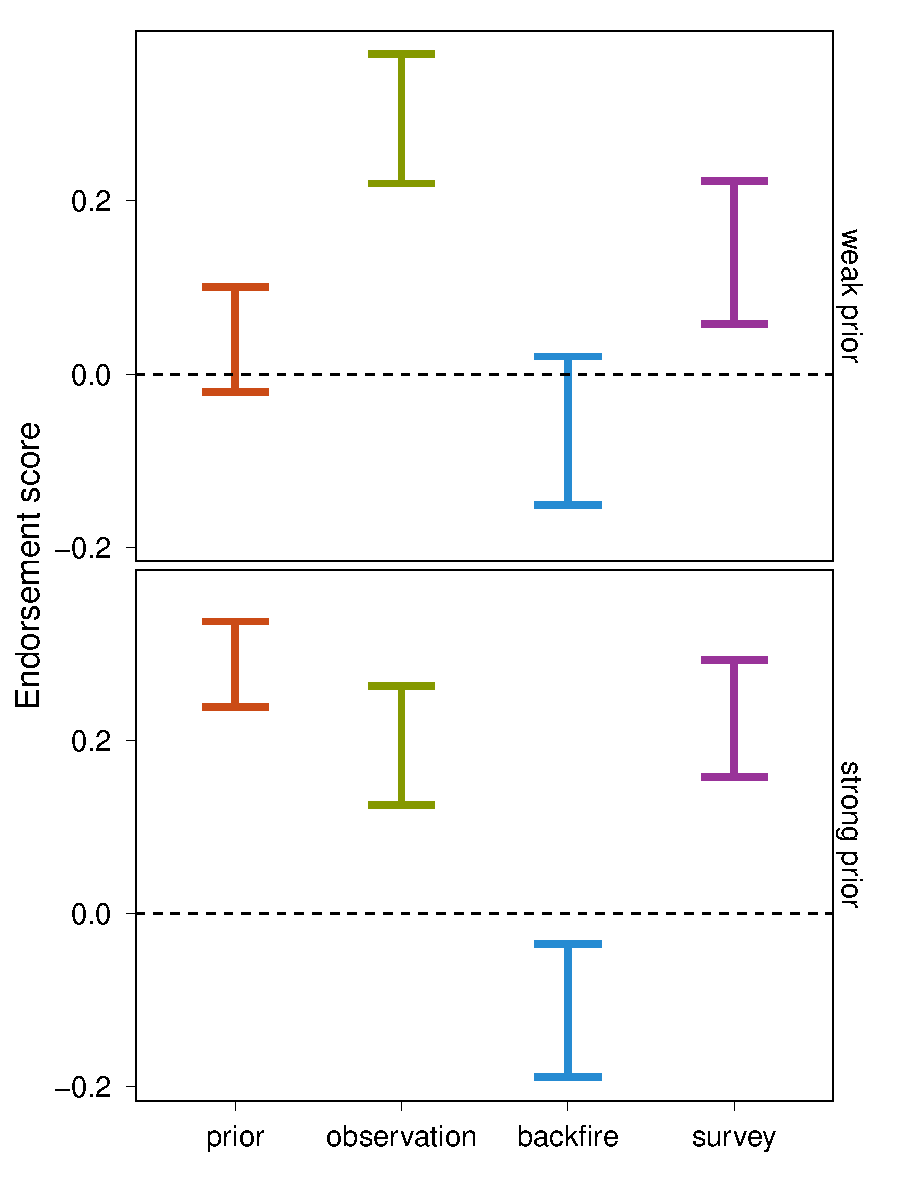
\includegraphics[width=\columnwidth]{fc2-score-medSplit}
    \caption{}
  \label{fig:expt1score}
\end{figure}

We report the results in terms of the proportion of participants who selected the \emph{likely} option (e.g. \emph{always does her dishes}). Additionally, we report the endorsement score, which incorporates the confidence ratings by scaling the response (either +1 or -1) by confidence. 

To determine how the Pragmatic, Literal, and Speaker Manipulation conditions compared to the Baseline condition, we fit the data using mixed-effects regression models comparing the responses and confidence ratings of the experimental conditions to those of the Baseline condition.  Each model had a fixed effect of condition and random effects of item and participant.  To test for the significance of effects, we performed likelihood ratio tests. Chi-squared values, degrees of freedom, and p-values, all from the likelihood ratio test, are reported for each statistical test.

As predicted, participants were significantly less likely to choose the "likely"€ option in the Pragmatic condition (M = .46, SE = XX, n = XX) than in the Baseline condition (M = .71, SE = XX, n = XX) , χ2(1) = 81.15, p < .001.  Reading, for example, "My student turned in his homework on time today,"€ in a communicative context caused participants to infer that the student does not typically turn in his homework on time.  Adults were also more confident in their choices in the Pragmatic condition (M = .63, SE = XX, n = XX) than in the Baseline condition (M = .39, SE = XX, n = XX).

The Literal (M = .71, SE = XX, n = XX) and Speaker Manipulation (M = .68,  SE = XX, n = XX) conditions, however, did not differ significantly from the Baseline condition, χ2(1) = 0, p = .98, and χ2(1) = 2.11, p = .15, respectively, even though we expected participants in these conditions to be more likely to choose the "likely"€ option.  One possibility is that for the items in this task, there was not much room for preference for the "likely"€ option to strengthen, given that participants already preferred the "likely"€ option in the Baseline condition at above-chance levels, t(119) = 9.05, p < .001.  Confidence ratings, however, did distinguish among these conditions.  Confidence ratings in both conditions (M = .60, SE = XX, n = XX in the Literal condition; M = .60, SE = XX, n = XX in the Speaker Manipulation condition) were significantly higher than confidence ratings in the Baseline condition,  χ2(1) = 275.41, p <.001, and χ2(1) = 255.68, p < .001, respectively.  Thus, the evidence provided in these two experimental conditions made adults at least more confident in their choices.  

POST-HOC ANALYSES?
To determine how pre-existing biases might influence participants'€™ responses in each of our conditions, we performed a median split analysis, separating items in the Baseline condition for which participants had weak preferences (M  = XXXX) from those for which participants had strong preferences (M = XXXX).  


%\section{Experiment 2} 
%Experiment 1 demonstrated the existence of a backfiring effect as a speech-act of what would usually be construed of as positive evidence: the observation of an event. 
%In Experiment 2, we explore downstream consequences of this inference. 
%If intuitive, structured theories of world are what guide inference, then we would expect to observe the effects of backfiring in different components of that structured konwledge.
%For example, If habits have a causal dependence on some more abstract trait, then having one's belief shaken in a person's habit can have belief shaken in the upstream trait. 
%For instance, upon hearing one's friend say \emph{My roommate did her dishes today.}, a hearer could plausibly infer both this an irregular event and that the roommate is the kind of person who wouldn't normally do her dishes. 
%That is, the roommate's room might also be a mess, she might be an inconsiderate person, or maybe more likely than not to fall delinquent on her rent checks.

%This opens the door for manifestly different types of conceptual learning from language. \red{This is a good point, but I feel like we'll end up focusing *not* on language (and instead on the relation between irregular events and traits)... which maybe is ok, I don't know.}


%and conceptually replicates \citeA{Kravtchenko2015} 


\section{General discussion}

We have replicated previous findings that adults interpret utterances so that they are not redundant with the listener's preexisting beliefs, based on the conversational agreement that utterances should be maximally informative (CITE).  Upon hearing, "My student turned in his homework on time today," for instance, adults will learn not only that the student turned in his homework on time, but also that the student must not typically turn in his homework on time.

We also expanded upon prior work in three important ways: 1) we developed a computational model that predicts this inferential process; 2) we demonstrated that adults do not make this inference when the listener's uncertainty about the event is in common ground with the speaker, or when the utterance is removed from a conversational context (i.e., when it is framed as an observation); and 3) we provide evidence that the strength of the backfiring effect systematically varies according to the adults' preexisting beliefs.

In addition to contributing to our knowledge of language processing, this work has practical relevance.  Recent efforts to persuade the general public that there is no causal relation between vaccines and autism, for example, include articles titled, "Vaccines do not cause autism" (e.g., CDC).  Similarly, websites, media outlets, and researchers tend to state, "Girls can do math," as a way of promoting gender equality (e.g., Smithsonian Mag).  While these two statements would certainly be useful and informative for those who \emph{do} believe that vaccines cause autism or for those who \emph{do not} believe that girls can do math, respectively, it is unclear how they might be received by people who already share these beliefs, or who are not aware of either of these debates.  The headline, "Girls can do math", for instance, could potentially signal to a number of readers that many people believe that girls cannot do math, and that there are legitimate reasons to hold this belief (e.g., perhaps girls tend to be less intelligent than boys).  As a result, these readers might walk away doubting girls' ability to do math more than they would have otherwise.

Of course, in the present study, our focus was on affirmations of past events (e.g., "My student turned in his homework on time"; "The gym had clean towels today"), as a first step towards modeling this backfiring effect of language.  Further work is therefore necessary to determine how other kinds of affirmations, such as generic claims, might also backfire.



\bibliographystyle{apacite}

\setlength{\bibleftmargin}{.125in}
\setlength{\bibindent}{-\bibleftmargin}

\bibliography{backfiring-cogsci2016}


\end{document}
